\documentclass[13pt,a4paper]{article}
\usepackage[spanish,es-nodecimaldot]{babel}	% Utilizar español
\usepackage[utf8]{inputenc}					% Caracteres UTF-8
\usepackage{graphicx}						% Imagenes
\usepackage[hidelinks]{hyperref}			% Poner enlaces sin marcarlos en rojo
\usepackage{fancyhdr}						% Modificar encabezados y pies de pagina
\usepackage{float}							% Insertar figuras
\usepackage[textwidth=390pt]{geometry}		% Anchura de la pagina
\usepackage[nottoc]{tocbibind}				% Referencias (no incluir num pagina indice en Indice)
\usepackage{enumitem}						% Permitir enumerate con distintos simbolos
\usepackage[T1]{fontenc}					% Usar textsc en sections
\usepackage{amsmath}						% Símbolos matemáticos
\usepackage[ruled,vlined]{algorithm2e}      % Pseudocódigo
\usepackage{xcolor}
\usepackage{listings}
% Para que acepten tíldes los listing
\lstset{     
     literate=%
         {á}{{\'a}}1
         {é}{{\'e}}1
         {í}{{\'i}}1
         {ó}{{\'o}}1
         {ú}{{\'u}}1
         {Á}{{\'A}}1
         {É}{{\'E}}1
         {Í}{{\'I}}1
         {Ó}{{\'O}}1 
         {Ú}{{\'U}}1
         {ñ}{{\~n}}1 
         {Ñ}{{\~N}}1 
         {¿}{{?``}}1 
         {¡}{{!``}}1
}
\usepackage{dsfont}

% ==============================================================================

\usepackage{caption, subcaption}
\usepackage[section]{placeins}
\makeatletter
\def\fps@figure{H}
\makeatother

\usepackage{booktabs}
\usepackage{longtable}
\usepackage{array}
\usepackage{multirow}
\usepackage{wrapfig}
\usepackage{colortbl}
\usepackage{pdflscape}
\usepackage{tabu}
\usepackage{threeparttable}
\usepackage{threeparttablex}
\usepackage[normalem]{ulem}
\usepackage{makecell}
\usepackage{xcolor}
\usepackage[bottom]{footmisc}

\makeatletter
\newcommand*{\centerfloat}{%
  \parindent \z@
  \leftskip \z@ \@plus 1fil \@minus \textwidth
  \rightskip\leftskip
  \parfillskip \z@skip}
\makeatother

% ==============================================================================
% ==============================================================================

% Comando para poner el nombre de la asignatura
\newcommand{\asignatura}{Visión por Computador}
\newcommand{\autor}{Ignacio Vellido Expósito}
\newcommand{\email}{ignaciove@correo.ugr.es}
\newcommand{\titulo}{Trabajo 1}
\newcommand{\subtitulo}{Sistemas de Visión Artifical}

% Configuración de encabezados y pies de pagina
\pagestyle{fancy}
\lhead{\autor{}}
\rhead{\asignatura{}}
\lfoot{Máster Ciencia de Datos e Ingeniería de Computadores}
\cfoot{}
\rfoot{\thepage}
\renewcommand{\headrulewidth}{0.4pt}		% Linea cabeza de pagina
\renewcommand{\footrulewidth}{0.4pt}		% Linea pie de pagina

% ==============================================================================
% ==============================================================================

\begin{document}
    \pagenumbering{gobble}
    % ==============================================================================
% Pagina de titulo
\begin{titlepage}
    \begin{minipage}{\textwidth}
        \centering

        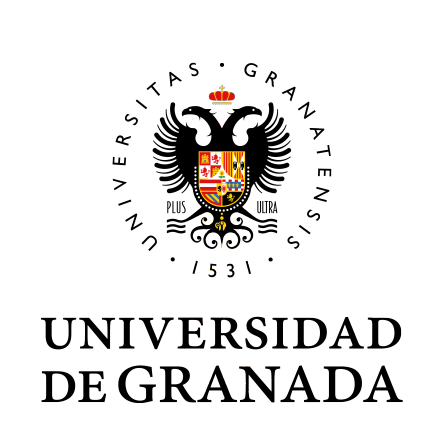
\includegraphics[scale=0.5]{img/ugr.png}\\

        \textsc{\Large \asignatura{}\\[0.2cm]}
        \textsc{MÁSTER CIENCIA DE DATOS E INGENIERÍA DE COMPUTADORES}\\[1cm]

        \noindent\rule[-1ex]{\textwidth}{1pt}\\[1.5ex]
        \textsc{{\Huge \titulo\\[0.5ex]}}
        \textsc{{\Large \subtitulo\\}}
        \noindent\rule[-1ex]{\textwidth}{2pt}\\[2.5ex]

        \end{minipage}

        \vspace{0.3cm}

        \begin{minipage}{\textwidth}

        \centering

        \textbf{Autor}\\ {\autor{} \\ ignaciove@correo.ugr.es}\\[1.5ex]
        \vspace{0.4cm}

        
\includegraphics[scale=0.3]{img/etsiit.jpeg}
        
\includegraphics[scale=0.6]{img/master.png}

        \vspace{0.7cm}
        \textsc{Escuela Técnica Superior de Ingenierías Informática y de Telecomunicación}\\
        \vspace{1cm}
        \textsc{Curso 2020-2021}
    \end{minipage}
\end{titlepage}
% ==============================================================================
    
    % \pagenumbering{arabic}
    % \tableofcontents
    % \thispagestyle{empty}				% No usar estilo en la pagina de indice

    \newpage

    % ==============================================================================

    \section{Introducción}

\subsection{Historia}

% Historia de los sistemas de visión artificial.Inspiración en la visión humana. Elementos que constituyen un sistema de visión artificial.

\begin{figure}[h]
  \centerfloat
  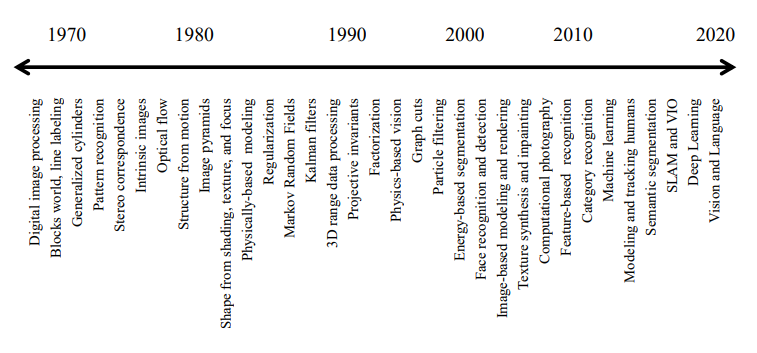
\includegraphics[width=0.75\textwidth]{img/history.png}
  \caption{Eventos destacables en la historia de la visión artificial.}
\end{figure}

La visión artificial comienza a plantearse en los años 60, después de que Larry Roberts propusiera la extracción de información geométrica a partir de fotografías 2D.
Sus primeras aproximaciones trataban tareas específicas como la detección de bordes o la identificación de patrones, basándose en técnicas matemáticas rigurosas.
Durante los 80 sigue el énfasis en explorar las distintas técnicas matemáticas y se plantean primeras ideas de CNN. Entre alguna de las aplicaciones se comienzan a usar las pirámides para la mezcla y para el manejo de imágenes multi-escala.
En los 90 surge un mayor esfuerzo en resolver problemas de movimiento. También aumenta el número de aplicaciones relacionadas con gráficos, como la modelización y representación de imágenes 3D.

\vspace{\baselineskip}

A comienzos del siglo XXI cambia la aproximación clásica de crear buenos modelos matemáticos con características cuidadosamente extraídas por un enfoque en el aprendizaje de características a partir de los datos bajo la asunción de que múltiples conceptos son compartidos. Entre algunas de las aplicaciones está primer framework de detección de caras a tiempo real (Viola-Jones) y el inicio de la experimentación con coches autónomos.

\vspace{\baselineskip}

Durante la década pasada sigue la tendencia de usar grandes bases de datos para desarrollar algoritmos de aprendizaje, y en 2012 comienza la expansión del aprendizaje profundo cuando la arquitectura AlexNet gana la competición ImageNet. A partir de entonces se diversifica el uso de la visión artificial en múltiples campos diferentes, la mayoría basándose en el potencial de estas nuevas técnicas.

% 60s: La visión artificial comienza a plantearse en los años 60, después de que Larry Roberts propusiera la extracción de información geométrica a partir de fotografías 2D.

% 70s: Los primeros intentos pretendían la detección de bordes y la identificación de patrones.

% 80s: Se comienza a aplicar un mayor énfasis en técnicas matemáticas y se plantean primeras ideas de CNN. Se comienzan a usar las pirámides de imágenes para la mezcla de imágenes y para el manejo de imágenes multi-escala.

% 90s: Múltiples esfuerzos en resolver problemas de movimiento y en la modelización y representación de imágenes 3D.

% 00s: Mayor influencia de los sistemas de aprendizaje dirigidos por datos. Surge una tendencia a aplicar técnicas basadas en características para la clasificación de objetos. Se introduce el primer framework de detección de caras a tiempo real (Viola-Jones). Google comienza su experimentación con coches autónomos

% Cambia la aproximación clásica de crear buenos modelos matemáticos con características cuidadosamente extraídas por un enfoque en el aprendizaje de características a partir de los datos bajo la asunción de que múltiples conceptos comparten características.

% 10s: Sigue la tendencia de usar grandes bases de datos para desarrollar algoritmos de aprendizaje. Se expande el uso de de reconocimiento de caras (redes sociales, seguridad\dots).


\begin{figure}[H]
    \centerfloat
    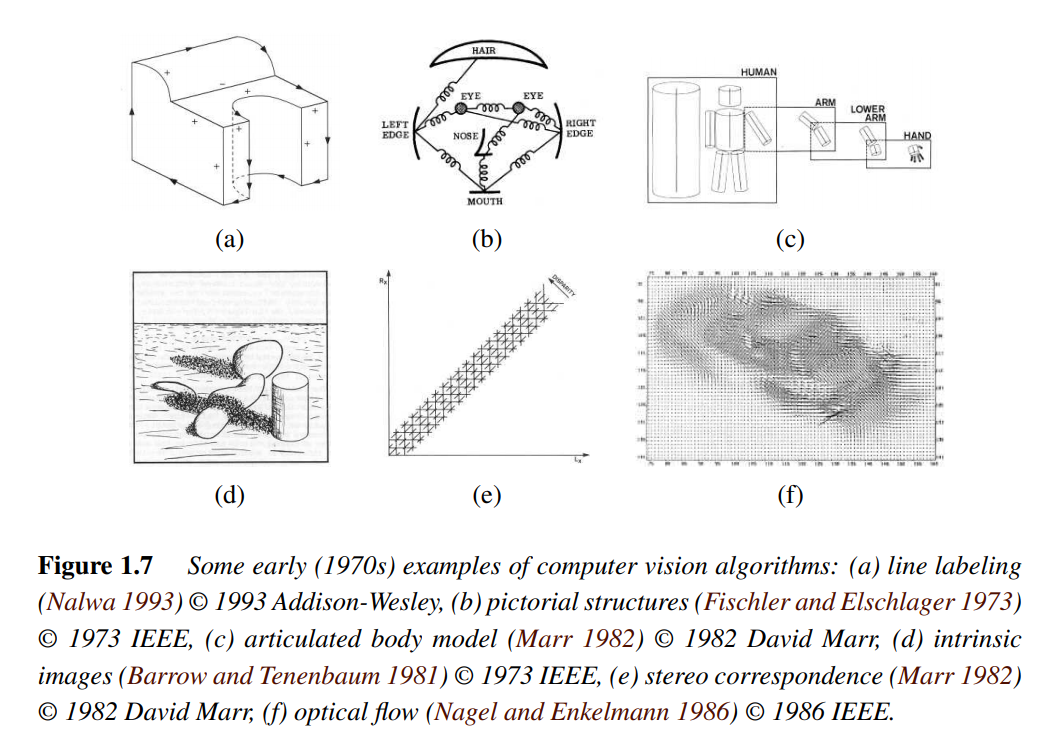
\includegraphics[width=0.75\textwidth]{img/70s.png}
\end{figure}

\begin{figure}[H]
    \centerfloat
    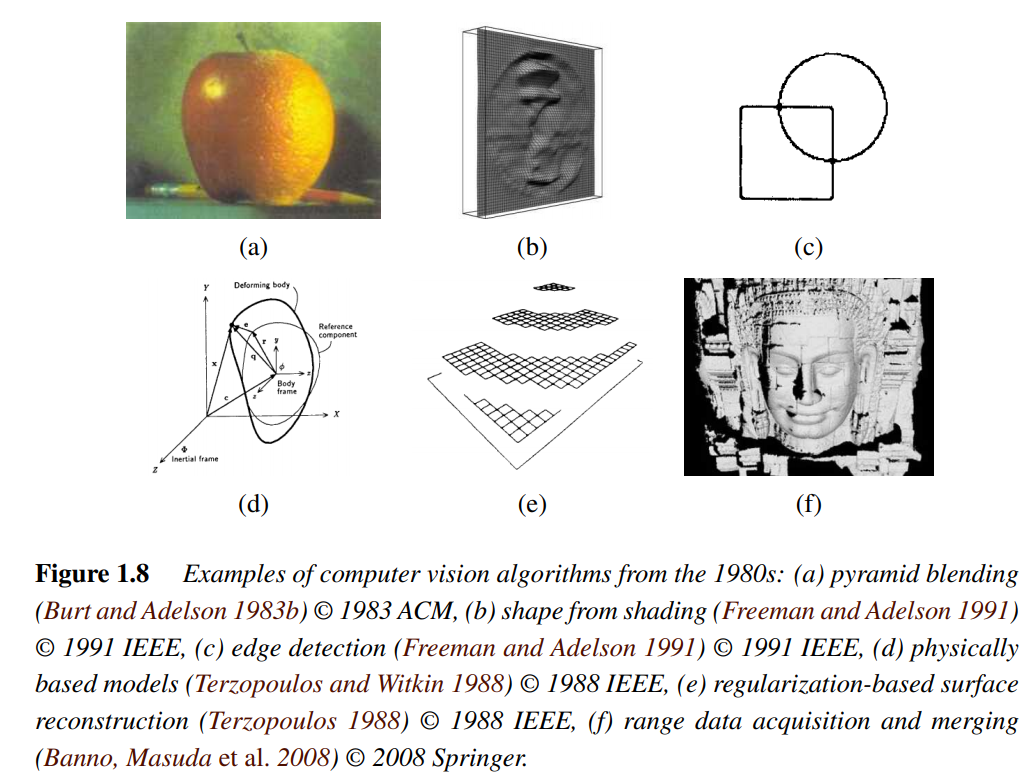
\includegraphics[width=0.75\textwidth]{img/80s.png}
\end{figure}

\begin{figure}[H]
    \centerfloat
    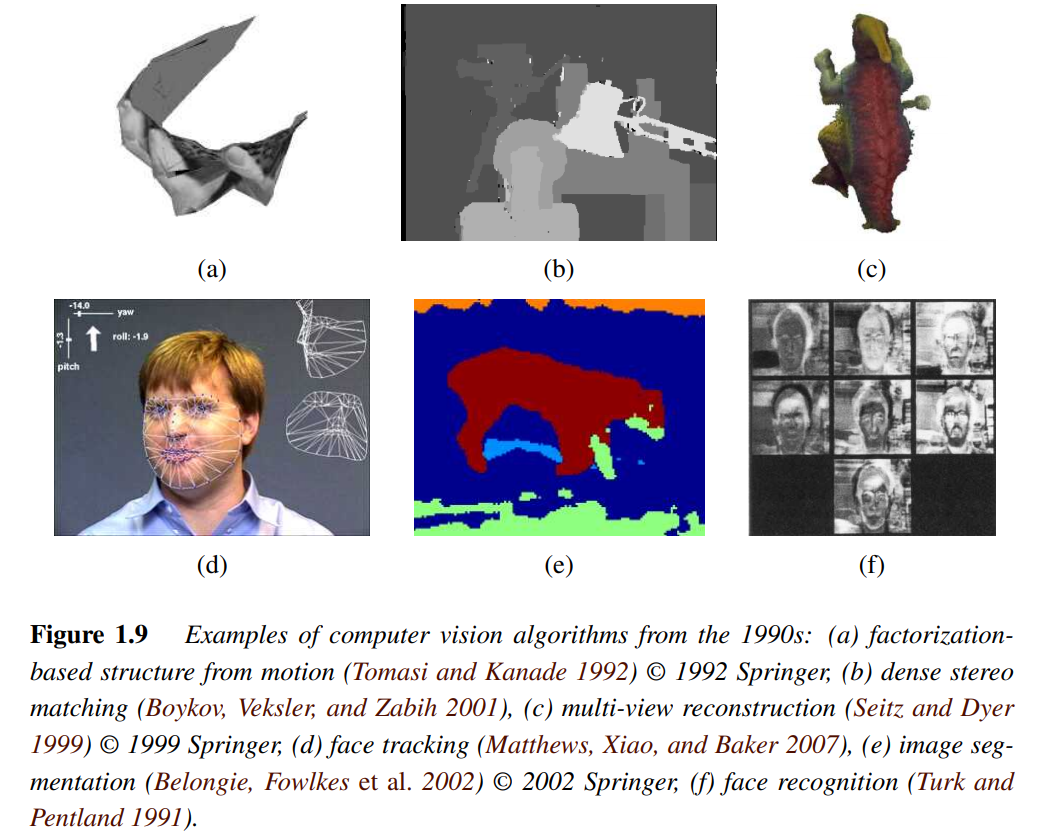
\includegraphics[width=0.75\textwidth]{img/90s.png}
\end{figure}

\begin{figure}[H]
    \centerfloat
    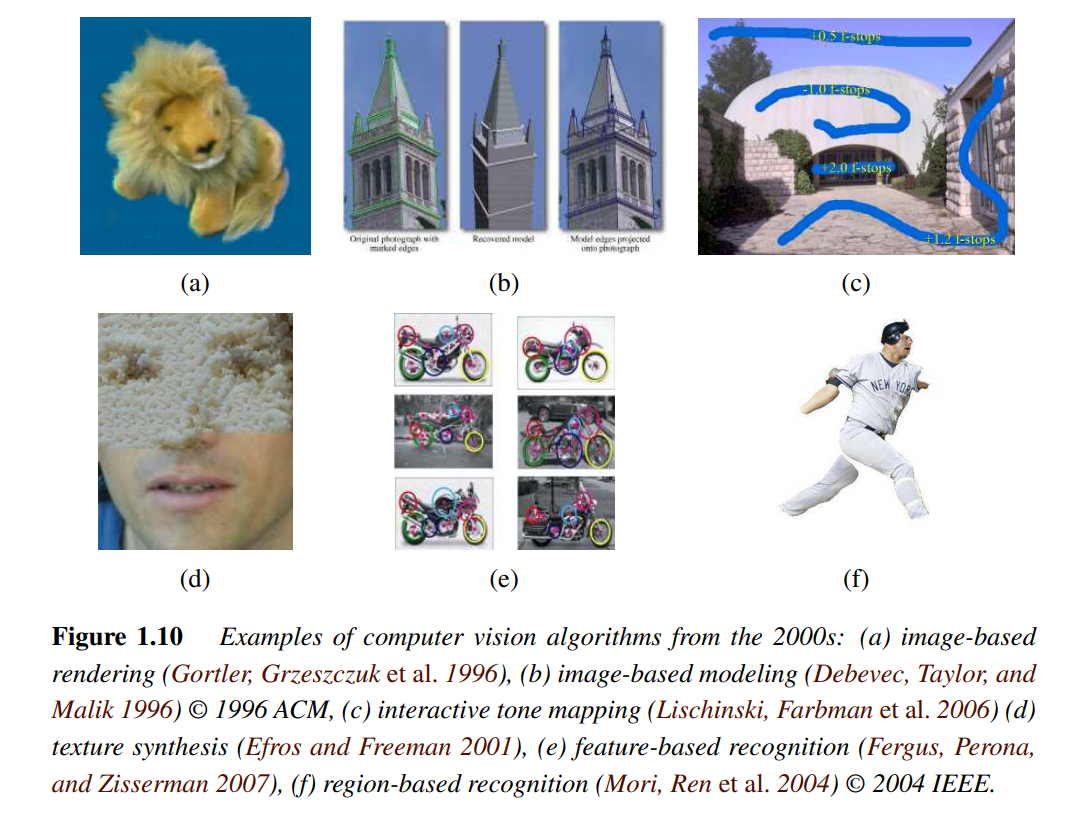
\includegraphics[width=0.75\textwidth]{img/00s.png}
\end{figure}

\begin{figure}[H]
    \centerfloat
    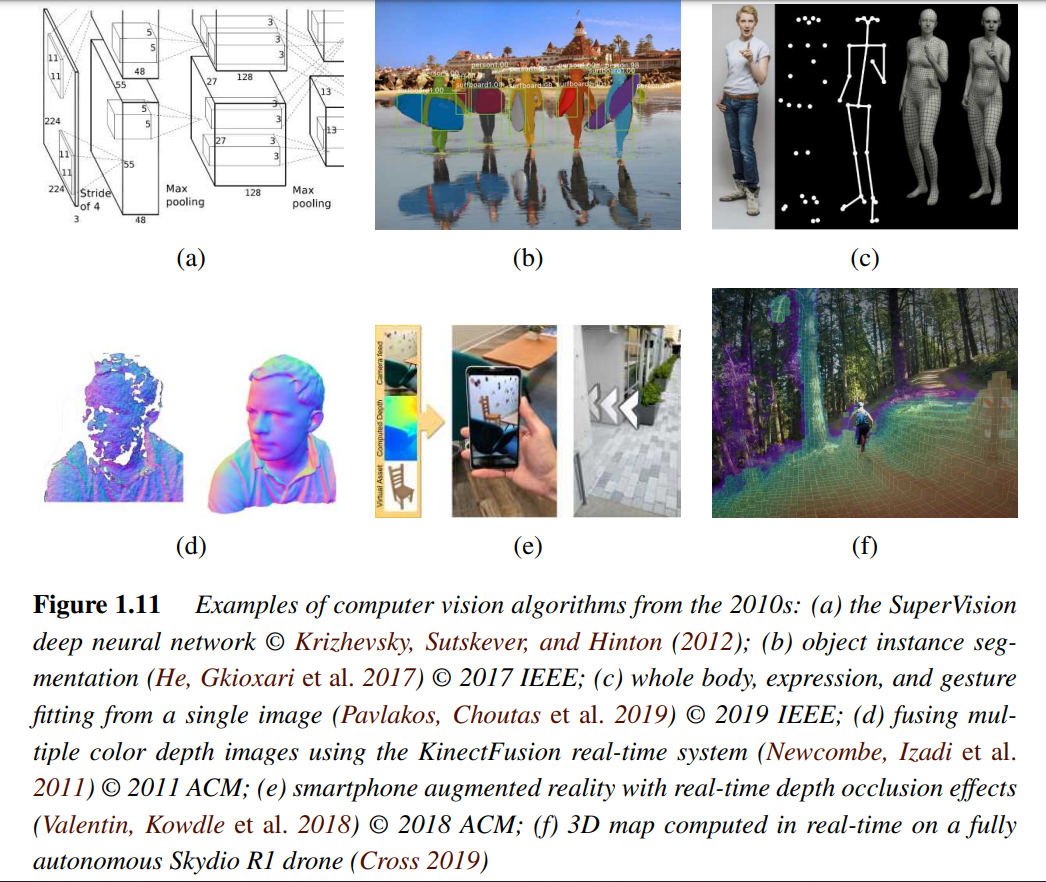
\includegraphics[width=0.75\textwidth]{img/10s.png}
\end{figure}

\subsection{Elementos}

Podríamos decir que los sistemas de visión por computador tienen en común:
Un sistema de captación y/o almacenamiento de imágenes, ya sea un físico (ej: cámara, escáner) o virtual (ej: recuperación de imágenes de internet).
Un sistema de preprocesamiento y adecuación de las imágenes para su uso.
La aplicación de técnicas para la extracción de información a partir de las imágenes. 
Realizar un proceso o tarea a partir de la información extraída, ya sea razonar o actuar (ej: vehículo autónomo), o generar una salida (ej: detección de objetos)

\subsection{Inspiración humana}

En términos generales el ojo y el cerebro humano son las fuentes principales de inspiración en la visión artificial, pero al haber aún mucho desconocimiento sobre el funcionamiento de este último siguen utilizándose técnicas matemáticas basadas en los pixeles de la imagen.

Existe también inspiración humana en la funcionamiento de las CNN. El ojo humano detecta características geométricas de bajo nivel (líneas, bordes, esquinas) con las que jerárquicamente va identificando el objeto. Esto mismo se ha visto modelado en las capas de una CNN a diferentes profundidades. Además, estas características básicas son comunes entre objetos, y son las diferentes formas de combinarse las que los distinguen los unos de los otros. \newpage
    \section{Estado del arte}

% \begin{figure}[h]
  %   \centerfloat
  %   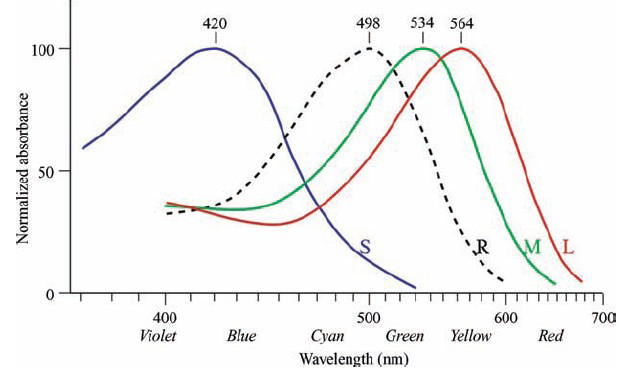
\includegraphics[width=0.75\textwidth]{img/conos.png}
  %   % \caption{Relación intermediación-vector propio en escala logarítmica.}
  % \end{figure} \newpage
    \section{Desarrollo de una aplicación}

% Escoger una aplicación real y describir como se hace en cada etapa. Las etapas que debemos abordar son:
%       Adquisición de las imágenes o video
%       Preprocesamiento
%       Segmentación
%       Extracción de características
%       Clasificación

Vamos a describir el proceso de desarrollo del sistema de visión de un supuesto robot terapéutico, capaz de detectar y hablar a la cara de una persona. Adicionalmente buscamos poder identificar personas o clasificar expresiones faciales.
% Existen diferentes formas de afrontar este problema, por un lado podríamos separar el problema en dos partes (localización y seguimiento de objetos, y detección de caras)
\begin{enumerate}
    \item \textbf{Adquisición}: El sistema de detección de caras debe incluir una cámara de vídeo de calidad suficiente para distinguir objetos en la escena. Puesto que vamos a aplicar técnicas de aprendizaje sobre las caras encontradas, necesitamos además una resolución buena y una buena capacidad de zoom (dependiente de la altura del robot).
    
    Adicionalmente, puesto que no se espera que los objetos en la imagen se muevan a alta velocidad, no es necesario contar con un framerate alto.

    Otra posible opción sería acompañar la cámara de vídeo con otro de tipos de cámaras no independientes de la luminosidad. Esto nos forzaría a luego traspasar las regiones detectadas a la imagen normal, y por simplicidad vamos a suponer en este caso que contamos con una única cámara.

    \item \textbf{Preprocesamiento}: Para facilitar la tarea de aprendizaje sería conveniente eliminar ruido de la imagen y ajustar el contraste de la imagen en base a las condiciones luminosas de la escena. Una forma simple con la que empezar podría ser un equalización de histograma, pero se podrían utilizar otras técnicas más complejas y adaptativas, por ejemplo haciendo uso de otros sensores que pudiera contar el robot.
    
    Según el tipo de aprendizaje que vayamos a utilizar podría sernos útil una representación solo de bordes de la imagen. En este caso vamos a suponer que tenemos datos suficientes y podemos utilizar técnicas de deep learning donde los detalles y colores de la imágen nos son útiles.

    \item \textbf{Segmentación}:
    Podría ser interesante poder segmentar los objetos del fondo, de cara a facilitar la tarea de aprendizaje.
    
    % Necesitamos por un lado ser capaces de distinguir las personas del resto de objetos en la escena, y una vez ahí separar la cara del resto del cuerpo 
    
    % La orientación de la cara debe ser relevante. Es importante poder reconocer una cabeza desde cualquier ángulo, y poder mantener un seguimiento de su ubicación cuando se rota alrededor de ella.
    
    % No necesitamos segmentar cada pixel de la imagen, solo la región espacial en la que se ubica la cara.

    \item \textbf{Extracción de características}:
    Podemos utilizar redes profundas como YOLO, donde no es necesario extraer características previas de la imagen. Por contrapartida esta red nos fuerza a que una vez tengamos las regiones de interés donde se encuentran las caras debamos comparar con frames anteriores para detectar cuál de estas regiones corresponde a la que estaba centrada el robot, de cara a no perder el ``interés'' de una cara por otra.

    Otra forma sería extraer las regiones aparte y luego aplicar un entrenamiento sobre cada una de ellas. En este caso sería importante no perder la localización espacial de la región y que la técnica de aprendizaje sea flexible en el tamaño de estas.

    También se podrían considerar usar descriptores de características como histogramas de gradientes orientados.
    
    \item \textbf{Entrenamiento}:
    En cualquiera de los casos tratamos con técnicas de aprendizaje supervisado, por lo que necesitamos datos lo más representativos posibles.

    Una vez obtenidas las regiones de interés podríamos llevar más allá el sistema realizando aprendizajes adicionales sobre ella, como identificación de personas o clasificación de sentimientos. En este caso probablemente la primera opción a considerar sería una red convolucional pre-entrenada del estado del arte, sobre la que podríamos aplicar transfer learning y fine tuning.

    Por último, el sistema de tracking debe poder retroalimentar los actuadores del robot para volver a centrar la cara. Esto se podría realizar fácilmente segmentando la imagen en forma de brújula e indicando en qué sector se ubica la cara.
\end{enumerate}

% 3. Como ejemplo: Sistema de CV: Reconocimiento de matrículas de coche
% Módulos (habría que desarrollarlos):
% - Adquisición: Cámara (y características). No dependiente de la luminosidad: Infraroja. Múltiples para captar varios ángulos
% - Preprocesamiento: Eliminación de ruido, añadiendo contraste. Cálculo de límites de los objetos
% - Segmentación: El coche del fondo, la matrícula del coche, cada carácter de la matrícula
% - Extracción de características (a no ser que se use convolución): Histogramas de orientación de gradiente, entropía, información de las fronteras...
% - Clasificación: SVC, KMeans, RNN, CNN (extraen características a la vez que clasifican). Supervisado, no supervisado...

% Los módulos pueden estar conectados a una base de conocimiento (con el dominio del problema) que indique lo que debe hacer cada uno.

    % Una vez tengamos ubicada la cara, deberíamos extraer las características de las esquinas de forma que podamos comprender y reorientar la cámara si la persona se mueve, aplicando un sistema de tracking entre sucesivos frames.

        % La clasificación de una cara puede ser aprendida usando técnicas de aprendizaje supervisado, siendo probablemente la primera opción a considerar una red convolucional, ya que para este caso es muy probable que una aplicación de transfer-learning con una red del estado del arte de buenos resultados.

            % Para la localización de la ubicación de la cara en la imágen sería conveniente tener una representación solo de bordes de la imagen, que nos permita distinguir los objetos ?.

\vspace{\baselineskip}
\vspace{\baselineskip}

Bibliografía:
\begin{itemize}
    \item Computer Vision: Algorithms and Applications, 2nd ed. 2021 Richard Szeliski
    \item Computer Vision: Evolution and Promise. T. S. Huang
    \item \url{https://en.wikipedia.org/wiki/Computer_vision}
    \item \url{https://www.verdict.co.uk/computer-vision-timeline/}
    \item \url{https://en.wikipedia.org/wiki/Pyramid_(image_processing)}
    \item Presentaciones de la asignatura: Visión por Computador. Nicolas Perez de la Blanca Capilla
    \item Presentaciones de la asignatura: Aplicaciones de Ciencia de Datos. Pablo Mesejo
    \item \url{https://en.wikipedia.org/wiki/Match_moving}
    \item \url{https://www.cs.ubc.ca/~lowe/vision.html}
\end{itemize}

    % ==============================================================================

    \setlength{\parskip}{1em}
    \newpage
    % \nocite{*}
    % \bibliography{bibliografia}
  	% \bibliographystyle{plain}
\end{document}